% Findings filed 22 November 2026 (report version 2.1)
\section{Detailed findings filed in this version (22 November 2026)}

These three findings came from a second round aimed at engineering results rather than input handling: hand calculations with the program's own IRC~6 vehicle tables, a span metamorphic test, physics oracles on design-check capacities, and fault injection in report generation. Each was reproduced in two fresh processes. All 210 upstream issues (open and closed) were searched for duplicates first.

% ---- 211
\subsection{\issue{211} --- Design live load taken from vehicles parked at $x = 0$}
\textbf{Severity / tier:} \sevH\ / T1. \quad \textbf{Proof:} \proof{211\_static\_vehicles\_fixed\_at\_x0/}

\textbf{Description.} \texttt{create\_governing\_ll\_load\_case()} (\texttt{analyser.py:1925}) selects the design live load only from the static vehicle cases (filter at line 1951). Every static vehicle is placed with its origin at the left support: \texttt{x\_coord = 0.0} (line 1641), applied at line 1834. The moving-load cases, which do traverse the span (lines 1908--1910), are not used for this selection. On a 40\,m span all static wheel loads lie in $x \in [0.6, 20.3]$\,m (2 $\times$ Class~A) and $[0.81, 13.75]$\,m (70R).

\textbf{Expected:} the live-load effect at the critical vehicle position. For a fixed set of vehicles, the maximum moment on a simply supported span increases with span.

\begin{center}\begin{tabular}{@{}lrrr@{}}
\toprule
40\,m span & Current ($x = 0$) & Vehicles centred & Change \\
\midrule
Governing LL $\max|M_z|$ & 1106.3\,kNm & 1527.7\,kNm & +38\,\% \\
LL moment per girder & 775--797\,kNm & 1362--1389\,kNm & +71--79\,\% \\
Design moment \texttt{mu\_applied} & 3553.9\,kNm & 4137.7\,kNm & +16.4\,\% \\
\bottomrule
\end{tabular}\end{center}

\textbf{Hand calculation.} Moment with the vehicle fixed at $x = 0$ divided by the moment at the worst position, single simply supported line: Class~A 0.89 / 0.90 / 0.84 / 0.71 and 70R 1.00 / 0.92 / 0.84 / 0.71 for spans 20 / 25 / 30 / 40\,m.

\textbf{Metamorphic check.} The program's live-load moment summed over the girders is 2240.4\,kNm (20\,m), 3216.4\,kNm (30\,m) and 3145.2\,kNm (40\,m): it \emph{decreases} from 30 to 40\,m.

\textbf{Fix (proven):} centring the static vehicles on the span (monkeypatch of the x offset only) gives the values in the right-hand column. Selecting the governing LL from the moving-load envelope would also fix it.

\begin{figure}[H]\centering
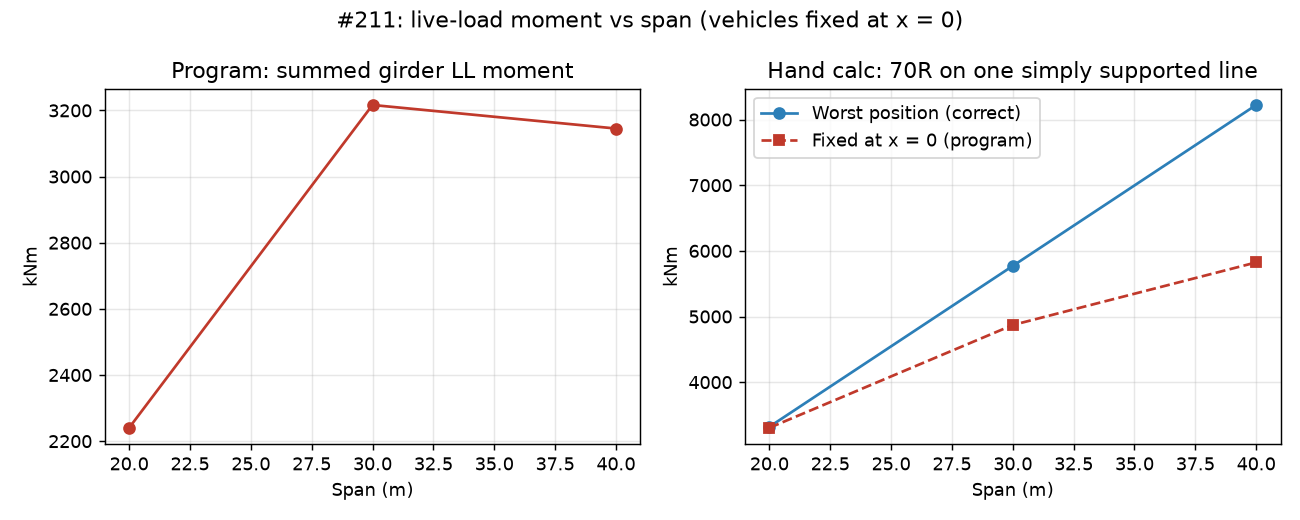
\includegraphics[width=0.92\linewidth]{../proofs/211_static_vehicles_fixed_at_x0/report_output/span_vs_ll_moment.png}
\caption{Left: program live-load moment against span (falls between 30 and 40\,m). Right: hand calculation for 70R, worst position against fixed at $x = 0$.}
\end{figure}

% ---- 212
\subsection{\issue{212} --- Older PDF returned as the new report when compilation fails}
\textbf{Severity / tier:} \sevM\ / T1. \quad \textbf{Proof:} \proof{212\_stale\_pdf\_returned\_as\_success/}

\textbf{Description.} \texttt{generate\_report()} judges success by \texttt{os.path.exists(pdf\_path)} in the output folder (\texttt{report\_generator.py:981--983}). The new PDF is copied there only if it was produced (lines 978--979). When compilation fails, a PDF left by an earlier report passes the check and is returned as the new report.

\textbf{Test.} A report for project PROJECTOLDA was generated normally; a second report for PROJECTNEWB was then generated into the same folder with \texttt{pdflatex} removed from \texttt{PATH} (child process only).

\textbf{Expected:} \texttt{pdf\_path = None} and an error. \quad \textbf{Actual:} \texttt{pdf\_path} returned as success; the PDF is byte-identical to the first one (same SHA-256 and modification time) and still shows PROJECTOLDA, while the new \texttt{.tex} contains PROJECTNEWB. The only trace is a log warning. Reproduced twice.

\textbf{Fix:} remove the old PDF before compiling, and test the PDF produced in the temporary folder together with the \texttt{pdflatex} return code.

\begin{figure}[H]\centering

\includegraphics[width=0.36\linewidth]{../proofs/212_stale_pdf_returned_as_success/screenshots/returned_pdf_page1_shows_PROJECTOLDA.png}
\caption{Title page of the PDF returned for project PROJECTNEWB: it still shows PROJECTOLDA.}
\end{figure}

% ---- 213
\subsection{\issue{213} --- Web-buckling capacity 69 times the squash load}
\textbf{Severity / tier:} \sevM\ / T1. \quad \textbf{Proof:} \proof{213\_web\_buckling\_exceeds\_squash\_load/}

\textbf{Description.} The check ``Brg.Stiff: Web Buckling'' (Cl.\,509.7.3.1) is, by its own comment, for the \emph{unstiffened} web bearing zone (\texttt{designer.py:1665}). Lines 1668--1670 compute the radius of gyration from the bearing-stiffener inertia divided by the bare-web area, and use the raw Euler stress $\pi^2 E/(KL/r)^2$ with no yield cap and no buckling curve. The stiffener column check next to it (line 1691) does use the program's design compressive-stress function.

\begin{center}\begin{tabular}{@{}lr@{}}
\toprule
Quantity (span 20\,m case) & Value \\
\midrule
Radius of gyration used (web alone: $t_w/\sqrt{12} = 2.31$\,mm) & 80.1\,mm \\
Reported stress $f_{cc}$ ($f_y = 350$\,MPa) & 21\,858.5\,MPa \\
Reported capacity (demand $R = 250.0$\,kN) & 109\,506\,kN, PASS \\
Squash load $A f_y/\gamma_{m0}$, $A = 5010$\,mm$^2$ & 1\,594\,kN \\
Program's own $f_{cd}$ for the web strut, $KL/r = 331$ & 14.7\,MPa $\Rightarrow$ 73.8\,kN, FAIL \\
\bottomrule
\end{tabular}\end{center}

\textbf{Expected:} a capacity not above the squash load; with the program's own function the unstiffened web fails, consistent with a bearing stiffener being provided. \quad \textbf{Impact:} the value is reported (design-check list and output dictionary) but does not drive another decision, because bearing stiffeners are checked separately. Reproduced twice.

\subsection{Extra evidence for existing issues}
\begin{itemize}[nosep]
  \item \issue{174} (combination factors): for the 20\,m case \texttt{BASIC\_1} (1.35\,DL) and \texttt{BASIC\_4} (1.0\,DL) give the same moment, 1092.872\,kNm; \texttt{mu\_applied} is 1141.8\,kNm against about 1705\,kNm by hand.
  \item \issue{104} (empty reactions table): the data behind the table is also wrong --- for every load case the left reaction equals minus the right, and only interior girders are summed (\texttt{results\_data.py:964--983}).
\end{itemize}
